\section{尾概率}
\label{sec:tail-events}

“至少$15$次正面”“响应超过$5$秒”“测量误差超过$0.1$”，这些事件有一个共同形状：随机变量落在某个阈值的一侧，或者离某个中心至少有给定距离。先把这类事件写成统一的形式，再看已知完整分布时怎样计算它们的概率。

\paragraph{单侧尾事件}
对随机变量$X$和实数$t$，事件$\{X>t\}$与$\{X\geq t\}$说的是$X$落在$t$的右边，事件$\{X<t\}$与$\{X\leq t\}$说的是落在左边。它们的概率都描述质量在一侧的残余，统称尾概率。

\begin{definition}[尾概率]
\label{def:tail-probability}
设$X$是随机变量，$t\in\mathbb{R}$。称
\begin{equation}
 \mathbb{P}(X>t),\qquad \mathbb{P}(X\geq t)
 \label{eq:tail-right}
\end{equation}
为$X$在$t$处的\term{右尾概率}（right tail probability），称$\mathbb{P}(X<t)$与$\mathbb{P}(X\leq t)$为左尾概率，二者统称\term{尾概率}（tail probability）。函数$t\mapsto\mathbb{P}(X>t)$称为$X$的\term{生存函数}（survival function）。
\end{definition}

“生存函数”的名字来自等待时间：若$X$是一个元件的寿命，$\mathbb{P}(X>t)$就是它活过时刻$t$的概率。这个函数从左到右不增，$t$趋于$+\infty$时趋于$0$。它下降得多快，就是本章所说的“尾部有多重”。

\paragraph{由分布函数计算}
分布函数$F_X(t)=\mathbb{P}(X\leq t)$直接给出两种尾概率：
\begin{equation}
 \mathbb{P}(X\leq t)=F_X(t),\qquad \mathbb{P}(X>t)=1-F_X(t).
 \label{eq:tail-from-cdf}
\end{equation}
后一个等式来自$\{X>t\}$是$\{X\leq t\}$的补事件。

带等号的右尾要小心。由第~\ref{chap:random-variables}章，分布函数在每一点有左极限，记作$F_X(t^-)=\lim_{s\to t^-}F_X(s)$，它等于$\mathbb{P}(X<t)$，跳跃高度$F_X(t)-F_X(t^-)$等于$\mathbb{P}(X=t)$。于是$\{X\geq t\}$作为$\{X<t\}$的补事件，概率是
\begin{equation}
 \mathbb{P}(X\geq t)=1-F_X(t^-)=1-F_X(t)+\mathbb{P}(X=t).
 \label{eq:tail-closed}
\end{equation}
只有当$X$在$t$处没有原子，即$\mathbb{P}(X=t)=0$时，才有$\mathbb{P}(X\geq t)=1-F_X(t)$。离散变量在可能取值处恰好有原子，这时把两者混用会差出整整一个点的质量。

\paragraph{贯穿例子}
掷$20$次均匀硬币，正面次数$X\sim\operatorname{Bin}(20,1/2)$，质量为
\[
 p_X(k)=\binom{20}{k}2^{-20},\qquad k=0,1,\dots,20 .
\]
由对称性$p_X(10+j)=p_X(10-j)$，只需列出$k\geq10$的一半。表~\ref{tab:tail-binomial}给出这些组合数，本章所有关于$X$的精确值都由这张表加出来，分母都是$2^{20}=1048576$。

\begin{BookInlineTable}
 \centering
 \caption{$X\sim\operatorname{Bin}(20,1/2)$在$k\geq10$处的组合数$\binom{20}{k}$，质量为$\binom{20}{k}/2^{20}$；$k<10$的部分由$\binom{20}{k}=\binom{20}{20-k}$得到。}
 \label{tab:tail-binomial}
 \begin{tabular}{rrrrrrr}
  \toprule
  $k$ & $10$ & $11$ & $12$ & $13$ & $14$ & $15$\\
  $\binom{20}{k}$ & $184756$ & $167960$ & $125970$ & $77520$ & $38760$ & $15504$\\
  \midrule
  $k$ & $16$ & $17$ & $18$ & $19$ & $20$ & \\
  $\binom{20}{k}$ & $4845$ & $1140$ & $190$ & $20$ & $1$ & \\
  \bottomrule
 \end{tabular}
\end{BookInlineTable}

至少$15$次正面的概率是最后六项之和：
\[
 \mathbb{P}(X\geq15)=\frac{15504+4845+1140+190+20+1}{2^{20}}=\frac{21700}{2^{20}}\approx0.02069 .
\]
严格多于$15$次则去掉$k=15$这一项：
\[
 \mathbb{P}(X>15)=\frac{6196}{2^{20}}\approx0.00591 .
\]
两者相差$p_X(15)=15504/2^{20}\approx0.01479$，比$\mathbb{P}(X>15)$本身还大。按式~\eqref{eq:tail-from-cdf}算出的$1-F_X(15)$是后者，不是前者。

图~\ref{fig:tail-binomial-tail}把这件事画了出来。左图的浅蓝柱是事件$\{X\geq15\}$包含的质量；右图是分布函数在$15$附近的阶梯，$15$处的竖直跳跃正是$p_X(15)$。$F_X(15^-)$取在跳跃下端，$F_X(15)$取在上端，用哪一个取决于端点是否算进尾事件。

\begin{BookInlineFigure}
 \centering
 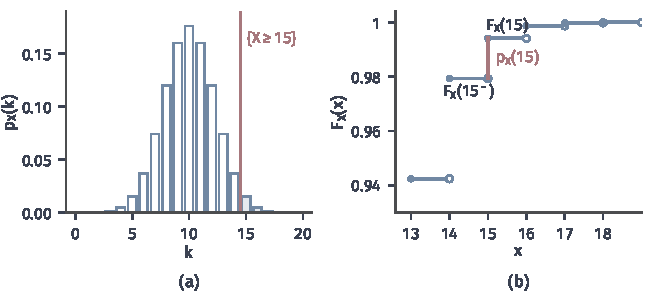
\includegraphics[width=112mm]{figures/07-probability/01-elementary-probability/matplotlib/tail-binomial-tail/figure.pdf}
 \caption{$X\sim\operatorname{Bin}(20,1/2)$的右尾。(a)质量表，浅蓝柱是事件$\{X\geq15\}$的质量，红线是阈值。(b)分布函数在$13$到$19$之间的阶梯，实心点是取到的值，空心点是左极限；红色竖线是$15$处的跳跃，高度为$p_X(15)$。}
 \label{fig:tail-binomial-tail}
\end{BookInlineFigure}

\paragraph{有密度的情形}
若$X$有密度$f_X$，单点概率为零，两种右尾相等，都等于密度在$t$右侧的面积：
\begin{equation}
 \mathbb{P}(X\geq t)=\mathbb{P}(X>t)=\int_t^{\infty}f_X(x)\,\mathrm{d}x .
 \label{eq:tail-density}
\end{equation}
三个模型足以展示尾部的不同衰减方式。$X\sim\operatorname{Exp}(1)$时积分得$\mathbb{P}(X>t)=\mathrm{e}^{-t}$，$t\geq0$。$Z\sim\mathcal{N}(0,1)$时右尾记作
\[
 Q(t)=\mathbb{P}(Z>t)=\int_t^{\infty}\frac{1}{\sqrt{2\pi}}\mathrm{e}^{-x^2/2}\,\mathrm{d}x ,
\]
它没有初等原函数，需要数值积分。常用的几个值是
\[
 Q(1)\approx0.1587,\quad Q(2)\approx0.02275,\quad Q(3)\approx0.00135 .
\]

第三个模型的尾部只按幂次衰减。对$\alpha>0$，在$[1,\infty)$上取密度$f_X(x)=\alpha x^{-\alpha-1}$，积分得
\begin{equation}
 \mathbb{P}(X>t)=\int_t^{\infty}\alpha x^{-\alpha-1}\,\mathrm{d}x=t^{-\alpha},\qquad t\geq1 .
 \label{eq:tail-pareto}
\end{equation}
令$t=1$得总质量为一，所以这确是密度。这个分布称为参数为$\alpha$的\term{Pareto分布}（Pareto distribution），$t<1$时$\mathbb{P}(X>t)=1$。本章用$\alpha=3$作为尾部较重的代表。

图~\ref{fig:tail-decay-shapes}把三条生存函数画在对数纵轴上。指数分布是一条直线，斜率为$-1$；高斯尾部向下弯，越来越陡，因为指数里是$t^2$；Pareto尾部越来越平，在$t=5$处仍有$0.008$，同一处高斯尾部已不到$3\times10^{-7}$。对数坐标把“远处还剩多少质量”的差别放大到了肉眼可见的程度。

\begin{BookInlineFigure}
 \centering
 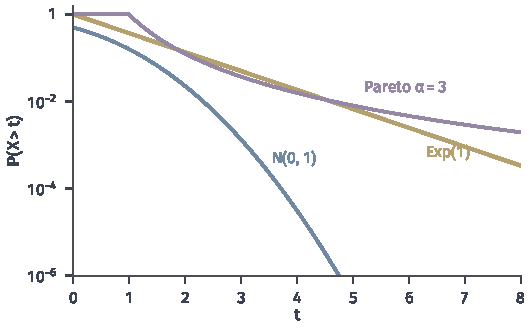
\includegraphics[width=90mm]{figures/07-probability/01-elementary-probability/matplotlib/tail-decay-shapes/figure.pdf}
 \caption{三种右尾，纵轴为对数刻度。蓝线为$\mathcal{N}(0,1)$的$Q(t)$，黄线为$\operatorname{Exp}(1)$的$\mathrm{e}^{-t}$，紫线为$\alpha=3$的Pareto分布的$\min\{1,t^{-3}\}$。}
 \label{fig:tail-decay-shapes}
\end{BookInlineFigure}

\paragraph{偏离中心的双侧事件}
很多时候关心的不是越过某个阈值，而是离某个中心$a$太远，例如测量值偏离真值至少$t$。对$t>0$，事件$\{\lvert X-a\rvert\geq t\}$拆成两个不相交的单侧事件：
\[
 \{\lvert X-a\rvert\geq t\}=\{X\geq a+t\}\cup\{X\leq a-t\} .
\]
两部分不相交，因为$a+t>a-t$。由加法规则和式~\eqref{eq:tail-closed}，
\begin{equation}
 \mathbb{P}(\lvert X-a\rvert\geq t)=1-F_X\bigl((a+t)^-\bigr)+F_X(a-t) .
 \label{eq:tail-two-sided}
\end{equation}
若$X$关于$a$对称，两部分相等，双侧概率是单侧的两倍。贯穿例子关于$10$对称，所以
\[
 \mathbb{P}(\lvert X-10\rvert\geq5)=2\,\mathbb{P}(X\geq15)=\frac{43400}{2^{20}}\approx0.04139 .
\]

分布不对称时两侧必须分开算。取$X\sim\operatorname{Exp}(1)$，均值为$1$，问偏离均值至少$t=0.5$的概率。左侧是$\{X\leq0.5\}$，右侧是$\{X\geq1.5\}$，分别为
\[
 \mathbb{P}(X\leq0.5)=1-\mathrm{e}^{-0.5}\approx0.3935,\qquad \mathbb{P}(X\geq1.5)=\mathrm{e}^{-1.5}\approx0.2231 .
\]
相加得$0.6166$，左侧贡献更大，见图~\ref{fig:tail-two-sided}。若$t\geq1$，左侧事件$\{X\leq1-t\}$要求$X\leq0$，概率为零，只剩右侧$\mathrm{e}^{-(1+t)}$。

\begin{BookInlineFigure}
 \centering
 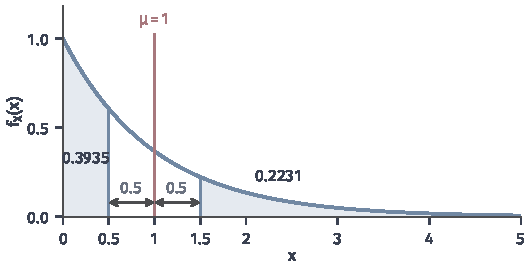
\includegraphics[width=90mm]{figures/07-probability/01-elementary-probability/matplotlib/tail-two-sided/figure.pdf}
 \caption{$X\sim\operatorname{Exp}(1)$偏离均值$\mu=1$至少$0.5$的事件。蓝线为密度，两块浅蓝区域是$\{X\leq0.5\}$与$\{X\geq1.5\}$，数字是各自的面积；红线标出均值。}
 \label{fig:tail-two-sided}
\end{BookInlineFigure}

\paragraph{尾概率与期望}
尾概率与期望之间有一条直接的联系。对非负整数值的变量，把$k\,p_X(k)$写成$k$个$p_X(k)$之和，再按“至少为$j$”重新归组：
\[
 \mathbb{E}[X]=\sum_{k\geq1}\sum_{j=1}^{k}p_X(k)=\sum_{j\geq1}\sum_{k\geq j}p_X(k)=\sum_{j\geq1}\mathbb{P}(X\geq j) .
\]
所有项非负，二重级数可以交换求和次序。对贯穿例子，把$\mathbb{P}(X\geq j)$对$j=1,\dots,20$相加，正好得到$10$。

有密度时，求和换成积分，并可以推广到$X$的函数。下面的\term{尾积分公式}说明期望完全由生存函数决定，后面检查矩与指数矩是否存在时要用它。

\begin{lemma}[尾积分公式]
\label{lem:tail-integral}
设$X\geq0$有密度$f_X$，$g$在$[0,\infty)$上连续可微且不减。则
\begin{equation}
 \mathbb{E}[g(X)]=g(0)+\int_0^{\infty}g'(s)\,\mathbb{P}(X>s)\,\mathrm{d}s ,
 \label{eq:tail-integral}
\end{equation}
两边同时有限或同时为$+\infty$。特别地，取$g(x)=x$与$g(x)=x^p$（$p>0$）得
\begin{equation}
 \mathbb{E}[X]=\int_0^{\infty}\mathbb{P}(X>s)\,\mathrm{d}s,\qquad \mathbb{E}[X^p]=\int_0^{\infty}p\,s^{p-1}\,\mathbb{P}(X>s)\,\mathrm{d}s .
 \label{eq:tail-integral-moments}
\end{equation}
\end{lemma}

\begin{proof}
由微积分基本定理，$g(x)-g(0)=\int_0^xg'(s)\,\mathrm{d}s$。两边乘$f_X(x)$并对$x\geq0$积分，得到
\[
 \mathbb{E}[g(X)]-g(0)=\int_0^{\infty}\Bigl(\int_0^{x}g'(s)\,\mathrm{d}s\Bigr)f_X(x)\,\mathrm{d}x .
\]
被积函数$g'(s)f_X(x)$在区域$0\leq s\leq x$上非负，所以可以交换积分次序，结果有限与否不受影响。交换的依据是非负函数的累次积分定理，可参考\BookChapterRef{chap:integration}{卷四第6章“积分”}；第~\ref{chap:probability-spaces}章会把它统一到概率的语言里。交换后内层对$x$从$s$积到$\infty$：
\[
 \mathbb{E}[g(X)]-g(0)=\int_0^{\infty}g'(s)\Bigl(\int_s^{\infty}f_X(x)\,\mathrm{d}x\Bigr)\mathrm{d}s .
\]
内层积分就是$\mathbb{P}(X>s)$，于是得到式~\eqref{eq:tail-integral}。
\end{proof}

用Pareto分布检验这个公式。$\alpha=3$时生存函数在$[0,1)$上为$1$，在$[1,\infty)$上为$s^{-3}$。代入式~\eqref{eq:tail-integral-moments}的第二式，对$0<p<3$，
\[
 \mathbb{E}[X^p]=\int_0^1p\,s^{p-1}\,\mathrm{d}s+\int_1^{\infty}p\,s^{p-4}\,\mathrm{d}s=1+\frac{p}{3-p}=\frac{3}{3-p} .
\]
$p=1$时得均值$3/2$，$p=2$时得$\mathbb{E}[X^2]=3$。若$p\geq3$，第二个积分发散，$p$阶矩为$+\infty$。尾部$s^{-3}$的衰减速度直接决定了哪些矩存在。

\paragraph{计算与估计}
已知完整分布时，尾概率是一个确定的数，按式~\eqref{eq:tail-closed}或式~\eqref{eq:tail-density}算出即可。反过来给定尾概率的水平去找阈值，就是第~\ref{chap:random-variables}章的分位数。直接计算的困难在于信息：很多时候只知道均值、方差之类的少数数值，或者完整分布虽然存在，却写不出可以求和、积分的形式。

这时能做的是给出\emph{上界}：找一个只依赖已知数值的量，保证所有具有这些数值的分布，其尾概率都不超过它。上界是一种保证，不是估计值；它必须对已知信息允许的最坏分布也成立。下面几节依次增加已知信息，看保证能收紧到什么程度。
